%-----------------------------------------------------------------------------
%
%               Template for sigplanconf LaTeX Class
%
% Name:         sigplanconf-template.tex
%
% Purpose:      A template for sigplanconf.cls, which is a LaTeX 2e class
%               file for SIGPLAN conference proceedings.
%
% Author:       Paul C. Anagnostopoulos
%               Windfall Software
%               978 371-2316
%               paul@windfall.com
%
% Created:      15 February 2005
%
%-----------------------------------------------------------------------------


\documentclass[10pt, conference, compsocconf]{IEEEtran}

% The following \documentclass options may be useful:
%
% 10pt          To set in 10-point type instead of 9-point.
% 11pt          To set in 11-point type instead of 9-point.
% authoryear    To obtain author/year citation style instead of numeric.

\usepackage{amsmath}
\usepackage{times}
\usepackage{epsfig}
\usepackage{subfigure}
\usepackage{balance}
\usepackage{color}
\usepackage{mdwlist}
\usepackage{fancyvrb}
\usepackage{graphicx}
\usepackage{cite}
\usepackage{paralist}
\usepackage{multirow}

%\newcommand{\kimsays}[1]{{\tiny{\bf\color{red} KIM SAYS: #1}}}

%%% deal with the footnote issue in tabular
\newcounter{myfootertablecounter}
\newcommand\myfootnotemark{%
    %\refstepcounter{footnote}%
\addtocounter{footnote}{1}%
    \footnotemark[\thefootnote]%
}%
\newcommand\myfootnotetext[1]{%
\addtocounter{myfootertablecounter}{1}
\footnotetext[\value{myfootertablecounter}]{#1}
}
% from now on, myfootnote has to be used rather than footnote to
% adapt the myfootercounter
\newcommand\myfootnote[1]{%
\addtocounter{myfootertablecounter}{1}
\footnote{#1}
}%

\usepackage{fancyvrb}
\DefineVerbatimEnvironment{code}{Verbatim}{fontsize=\scriptsize}

%\usepackage{simplemargins}
%\ifCLASSINFOpdf
%\else
%\fi

\normalsize
\pagestyle{plain}
\pagenumbering{arabic} 

\begin{document}
\linespread{.97}
\selectfont
\special{papersize=8.5in,11in}
\setlength{\pdfpageheight}{\paperheight}
\setlength{\pdfpagewidth}{\paperwidth}

\title{A Language and Compiler\\for Iterative Stencil Loops}
%\title{A Language and Optimizing Compiler for Iterative Stencil Loops}
%\subtitle{Subtitle Text, if any}

\author{Jeremy W.~Sheaffer, Gregory Faust, Salvatore Valente, Kim Hazelwood
  and Kevin Skadron\\
  \{jws9c, gf4ea, sv9wn, hazelwood, skadron\}@cs.virginia.edu\\\\
  Department of Computer Science Department, University of Virginia}

\maketitle

\begin{abstract}

%% Parallel hardware is now widely available, yet writing and optimizing
%% parallel programs using sequential languages is difficult and error prone.
%% Therefore, it is useful to consider new language constructs that make it
%% easier for programmers to express parallel applications without the need to
%% attend to all the complexity of writing parallel algorithms.  Here we present
%% a new language in which users can easily express computations that involve
%% iterative stencil calculations.  Such computations form an important subset
%% of parallel algorithms and are widely used in scientific, engineering, and
%% other important application areas.

We present a high-level language for iterative stencil loops called {\em
  Stencil Language} (SL).  Using SL, a programmer need only express the
central kernel of their computation, not an entire parallel program.  We have
also built a translator for SL capable of translating the SL program into
code for different parallel programming models.  We provide an initial
translation into optimized code for the C++ extensions of the CUDA
programming model for NVIDIA GPUs and for multi-node CUDA distributed with
MPI.  Our CUDA optimizer is an extension of a previously proposed analytical
model for CUDA stencil applications.  Our model improves over the previous
model by automatically utilizing both static and dynamic information about
the application and the specific GPU environment in which the application is
running.  This allows the optimized version of the application to be derived
without the need for the application developer to specify any
execution-environment specific information.  Finally, we provide results that
show that the code generated from SL for CUDA is up to $2.3\times$ faster
than na\"{i}ve CUDA code across six applications and two generations of
NVIDIA hardware.

\end{abstract}

%\category{CR-number}{subcategory}{third-level}
%\terms term1, term2
%\keywords keyword1, keyword2

\section{Introduction}

{\em Iterative stencil loops} (ISLs)~\cite{li} are a class of loops that are
commonly used in fields including numerical simulations and signal
processing.  ISLs compute a time varying set of values in an array.  The
value for each array element in each time step depends upon the value for
that element and a set of nearby elements from the previous time step.  The
pattern of neighboring elements is called the {\em stencil}.  This access
pattern means that each element in the current time step can be calculated
independently of all others.  Therefore, techniques that take advantage of
data parallelism are applicable to ISLs, and can often lead to dramatic
speedups over serialized implementations, yet implementing parallel ISLs
presents several challenges.

A typical implementation of a parallel ISL divides the array into {\em tiles}
and assigns one or more tiles to each processor.  A complication of this
technique is that elements near the edge of a tile may reside in a tile
assigned to another processor; therefore, a certain amount of data sharing
between otherwise disjoint tiles is required.  Furthermore, on architectures
with a high communication cost, an optimal ISL implementation allows each
processor to calculate several time steps on its tiles before requiring
communication.

To accommodate this communication delay, disjoint tiles must overlap.  The
amount of overlap increases with the number of time steps between
communication events.  Additionally, values of array elements in the
overlapping region must be redundantly calculated because each processor
needs the boundary values locally for intermediate time steps.  The correct
number of time steps to allow between processor synchronization is therefore
a trade-off between the cost of synchronization and the associated data
exchange, and the number of redundant values that are calculated.

These trade-offs are poorly understood and are highly architecture dependent.
They are particularly challenging on new accelerator processors with novel
memory hierarchies and synchronization support; GPUs are a prominent example,
having attracted great interest for general-purpose engineering and
scientific computing due to their high data-parallel throughput and low cost.

What is needed is a way for users to express ISL computation in a way that
allows them to focus on their application rather than the parallel
optimization techniques needed for performance.  In this paper, we discuss
our efforts to provide such a system.  Our contributions are as follows:

\begin{itemize*}
\item We have implemented SL, a formal, high-level language in which a
  programmer can describe an ISL computation.  By design, a description
  written in the language must include all of the information necessary to
  calculate the correct results, and none of the information that would tie
  its performance to a particular architecture.
\item We have created a front-end compiler for SL that can easily be extended
  with multiple back-ends.  Based on a single source file, produces code for
  CUDA~\cite{CUDA1, CUDA2}, Open\-MP~\cite{OpenMP} and MPI~\cite{MPI-2.2}.
\item Our CUDA code optimizer transparently calculates the optimal tile size
  and time steps between synchronizations, and takes advantage of scratchpad
  memory.  It extends the analytical model proposed by Meng and
  Skadron~\cite{meng}.
\item Our system automatically collects all the necessary application
  specific and execution environment information needed by the model.  Some
  is derived statically from the SL program, and the rest is derived
  dynamically at runtime.
\item Dynamic acquisition of the execution environment information allows the
  generated code to calculate good values on a variety of GPU cards.  We
  demonstrate this capability by reporting results on both the Tesla and
  Fermi architectures.
\end{itemize*}

\section{SL System Organization}

Figure~\ref{fig:SysOrg} shows the system organization and information flow of
the SL compiler.  The application programmer specifies an ISL computation in
an SL source file.  The remainder of their application is specified in C or
C++.  In a simple scenario, the application code configures the array upon
which the ISL will operate and calls the code generated by the SL compiler to
do the ISL computation.  The results of the ISL computation can then be used
by the application.  The SL compiler generates a C Header File for inclusion
in the application code to declare the signature of ISL subroutines.

Figure~\ref{fig:SysOrg} shows the general system organization.  The SL
compiler takes in two sources of information: the SL program and and SL
system template that includes hand optimized implementations of the general
structure of an ISL computation for various runtime environments.  The
templates are written by the SL system developers, not the SL user.  Based on
the user specified target environment, the SL compiler selects the
appropriate library template and modifies it to implement the user's stencil
calculation.  The SL compiler produces program source as output, essentially
a source-to-source process, which is linked with the user's application
source into a final executable.

Many scientific applications require multiple ISL computations in a pipeline.
This usage scenario is supported by our system.  Each ISL computation is
specified in its own SL source file.  The user's application code can then
call the generated subroutine for each ISL computation as needed.

\begin{figure}
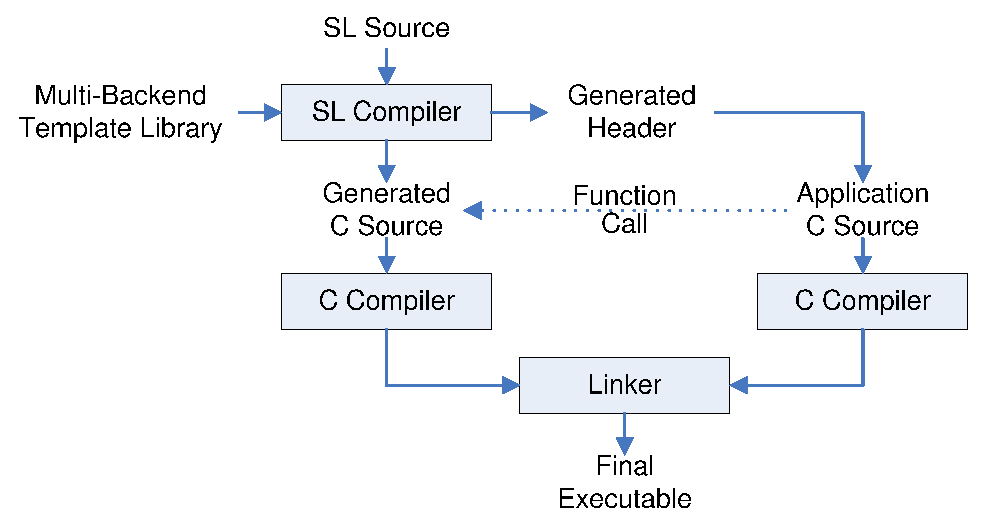
\includegraphics[width=\columnwidth]{figures/WorkFlow}
\caption{SL System Diagram showing information flow in SL.  The SL source is
  combined by the SL compiler with the appropriate optimized back-end
  template. The resultant generated subroutine for the ISL calculation is
  called by the rest of the user's application code.\vspace{-.20in}}
\label{fig:SysOrg}
\end{figure}

\section{Iterative Stencil Loops: Terms \& Background}

{\em Iterative stencil loops}~\cite{li} are a class of loops, commonly used in
numerical simulations and signal processing, which typically operate on
matrices with one, two, or three dimensions.  An ISL calculation takes an
input matrix $m_{in}$ and produces an output matrix $m_{out}$.  The
calculation has the following properties:

\begin{enumerate*}
\item $m_{in}$ and $m_{out}$ have the same number of dimensions and are the
  same size.
\item Each value in $m_{out}$ is calculated independently of each other value
  in $m_{out}$.
\item There is a single function which is used to calculate each value in
  $m_{out}$ regardless of the coordinates of the value.
\end{enumerate*}

For example, suppose $m_{in}$ is a two-dimensional matrix, and the stencil
calculation is defined as ``$m_{out}[x, y] =$ the average of the north,
south, east, and west neighbors of $m_{in}[x, y]$''.  Then this function will
be calculated for every cell in $m_{out}$.

The {\em stencil} is the set of cells in the input matrix that is used in the
stencil calculation, relative to the coordinates of the cell that is being
calculated.  In the above example, the stencil is a set of four cells: the
north, south, east, and west neighbors.

The process of calculating a complete output matrix is called an {\em
  iteration} or a {\em time step}.  At the end of an iteration, the output
matrix $m_{out}$ is used as the input matrix to the next iteration.  This
loop can continue for as long as necessary.  Some iterative stencil loops are
defined to run for a predetermined number of time steps, while others are
defined to run until the values converge.  Both cases are handled by SL.

Stencil calculations are data parallel.  Since each value in a time step is
calculated independently, the values can be calculated in any order.  If the
matrix has $n$ cells and the computer has $k$ {\em processing elements} (PEs)
available, then each processor only needs to calculate a block of size $n/k$.
This partitioning of the matrices among multiple processors is called {\em
  tiling}, and the block calculated by a PE is called a {\em tile}.

When a PE calculates a given tile for many iterations, that PE can take
advantage of both spatial locality and temporal locality.
\begin{itemize}
\item {\bf Spatial locality:} As a general rule, stencil calculations use each
  input value multiple times.  For example, given a stencil defined as a
  cell's left and right neighbors, when a PE calculates the cell value at
  $x=i$, it reads the value of the right neighbor at $x=i+1$.  When it
  calculates the cell value at $x=i+2$, it reads the left neighbor, the value
  at $x=i+1$ again.  Thus, a PE can optimize computation by keeping input
  values in a local cache or scratchpad.
\item {\bf Temporal locality:} If a PE generates an output value during
  iteration $t$, then that PE can use that value as an input value during
  iteration $t+1$.
\end{itemize}

Unfortunately, if each PE is given only those array values that fall within
its tile size, cells along the boundary of the tile will not find all of
their inputs in the local cache.  These cells must obtain some of their
inputs from array values assigned to other PEs.  In the example above, the
cell in the bottom left corner of a tile will require values for both its
south and west neighbors from neighboring tiles.  The region of data
surrounding a tile that is needed from adjacent tiles is called its {\em
  ghost zone} or GZ.

In order to take advantage of temporal locality, each PE may want to compute
more than one time interval with the array values it has stored locally;
however, at each successive time interval, more values at the periphery of
the PEs local store become stale.  For example, consider the 2D tile
computation shown in Figure~\ref{fig:trapezoid}(a).  It shows the shrinking
number of valid values calculated in a tile over four time intervals.  In the
first time interval, $i$, with a stencil size of one, the PE will require a GZ
of size one all around the periphery of the tile.  However, in calculating
the second time interval $i+1$, the values in the original GZ are still from
time $i$ and are now out of date.  Therefore, the PE is only able to
calculate a smaller number of valid values, and the size of the GZ has
expanded by the size of the stencil on all sides of the tile.  In the
diagram, this progression of stale values and expanding GZs will continue
inward through time interval $t+3$, after which only the inner most rectangle
will have valid values.

\begin{figure}
\begin{center}
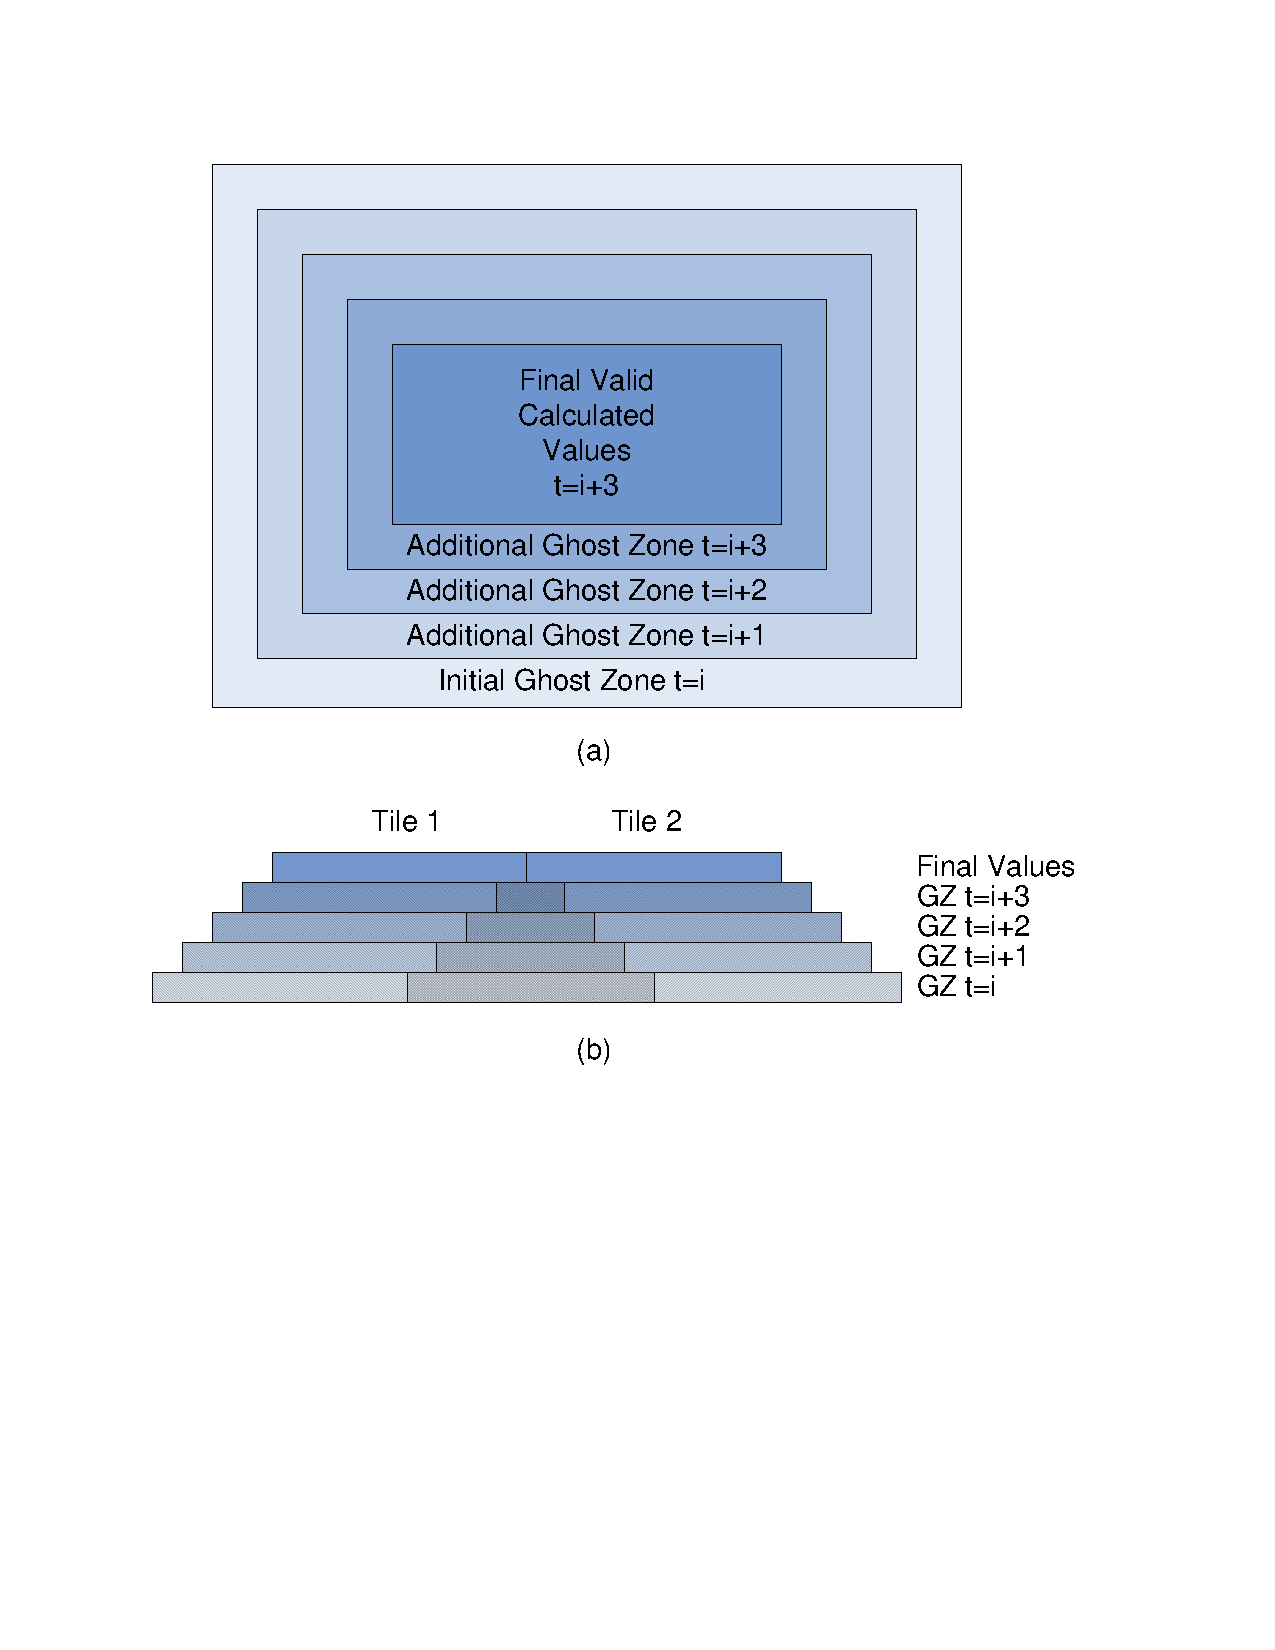
\includegraphics[width=.9\columnwidth]{figures/Diagrams}
\end{center}
\caption{(a) For a single tile in a 2D matrix, the number of valid calculated
  values decreases with each additional time interval between synchronization
  events.  After 4 time steps, only the inner most rectangle of $n$ values
  are valid.  (b) Two adjacent tiles shown from the plane of the 2D array
  with time in the vertical dimension.  In the first time step (bottom) there
  is substantial overlap in the ghost zones in order to have the resultant
  valid values abut after 4 time steps (top).\vspace{-.20in}}
\label{fig:trapezoid}
\end{figure}

Figure~\ref{fig:trapezoid}(b) shows the overlap in GZs between two adjacent
tiles for the same computation over four time intervals with time in the
vertical dimension.  Each PE must start with GZ size four in order to have
valid values computed for the resultant tiles cover the entire input array.
Because the size of the area of valid values for a PE shrink with time in
this way, the number of time intervals each PE calculates between
synchronization events is called the {\em pyramid height} or PH of the ISL.
In general, the size of the required GZ is equal to twice the size of the
stencil times the PH.  In addition, the values for cells in all but the
initial GZ are redundantly calculated by adjacent PEs.

As a result of the required data exchange between PEs, ISL algorithms may
spend considerable time stalled due to communication and synchronization
delays.  Because synchronization events can have high latencies, it is often
better to reduce the number of synchronizations between PEs by increasing the
PH and therefore the size of the GZ.  As we have seen, larger GZs result in
larger data exchanges at each synchronization and more redundant
calculations; therefore, the choice of the optimal PH for an ISL involves a
trade-off between these two competing costs and benefits.  The performance of
ISLs depends critically upon the correct choice.

There have been several attempts to optimize these trade offs, such as the
study by Meng and Skadron~\cite{meng} which examines the problem of writing
efficient ISL code in CUDA.  They define a mathematical model to calculate
the optimal PH for an ISL targeted for NVIDIA GPUs.  We have built upon the
results of that study, and have fully automated that optimization process in
our SL compiler.

\section{Stencil Language Description}

Figure~\ref{fig:hotspot} shows an SL description of the ``HotSpot''
calculation.  This code calculates temperature across a two-dimensional
micro\-chip where the current state is a function of the previous state, the
edge values, and a 2D read-only ``power usage'' matrix.  We will examine the
various aspects of this example in turn.

\begin{SaveVerbatim}{hs_code}
NumDimensions 2
StencilSize (1, 1)
DataType float
FunctionName runHotspot

ScalarVariables (
  float Rx, float Ry, float Rz
}
CellValue {
  float pvalue, value, term1, term2, term3, sum;
  pvalue = read(y * input_size.x + x);
  value = get(0, 0);
  term1 = (get(0, 1) + get(0, -1) - value) / Ry;
  term2 = (get(1, 0) + get(-1, 0) - value) / Rx;
  term3 = (80.0 - value) / Rz;
  sum = pvalue + term1 + term2 + term3;
  return(value + sum);
}
EdgeValue {
  return value;
}
\end{SaveVerbatim}

\begin{figure}
\begin{footnotesize}
\resizebox{\columnwidth}{!}{\BUseVerbatim{hs_code}}
\end{footnotesize}
\caption{The {\tt hotspot.sl} stencil language file.  This example shows a 2D
  stencil calculation where each cell value is based on the values of that
  cell's immediate neighbors.  The read-only data is interpreted as a 2D
  matrix in row-major order which indicates that some areas of the chip
  inherently run hotter then other areas.\vspace{-.20in}}
\label{fig:hotspot} 
\end{figure}

\subsection{Syntax}

A stencil language file is a text file that contains a set of key-value
pairs.  A key is an alphanumeric string.  A value can be:
\begin{itemize*}
\item an integer
\item a name comprised of alphanumeric and underscore characters
\item a list of names, inside parentheses, separated by commas
\item a block of code inside of curly braces
\end{itemize*}
\noindent We do not provide a grammar for SL as the key-value pairs are
sufficiently simple (constituting a regular language) as to obviate its need.
Technically, SL is only scanned, not parsed.  On a scan error, the system
prints an error message and aborts.  Other errors will be caught by the
backend compiler after the system makes substitutions into the backend
template; with the backend code used in the prototype, {\em \#line}
directives are inserted into generated source to aid the user with both
compile- and run-time errors.
\subsection{Content}

The currently supported SL keywords are:

\noindent {\bf NumDimensions:} A stencil may have 1, 2, or 3 dimensions.
\\\noindent {\bf StencilSize:} The size of the stencil in each dimension.  If the
  stencil size is 1 in the $x$ dimension, then the value of the cell at $(x,
  y)$ may be based on the previous iteration's values of the cells in the
  $x-1$ and $x+1$ coordinates.
\\\noindent {\bf DataType:} The value may be any valid integral type in the target
  language.
\\\noindent {\bf FunctionName:} The name of the function that will be exported
  from the generated source file.  The first argument to the function, {\tt
    data}, will be a matrix of the specified data type with the specified
  number of dimensions.  As input to the function, {\tt data} must contain
  the initial state of the problem.  It must contain valid data in each cell.
  As output from the function, it will contain the final data.  The next $n$
  arguments to the function are the input sizes in each dimension.  The next
  argument is the number of iterations to run.
\\\noindent {\bf ScalarVariables:} A list of numeric variables that will be
  arguments to the exported function after {\tt data, x, y, z, itera\-tions}.
  The caller will pass these arguments to the function, and then the stencil
  calculator will be able to use these variables (read-only) in its
  calculations.
\\\noindent {\bf CellValue:} A block of code that will be run for every cell in the data
  set in every iteration.  The code has access to the following variables and
  functions:
\begin{itemize*}
\item {\bf x, y, z:} Coordinates of current cell in each dimension.
\item {\bf iteration:} Iteration number.  Iteration 0 is given as input, so
  this code will first be called with {\tt iteration}=1.
\item {\bf input\_size:} a structure with {\tt x}, {\tt y}, and {\tt z}
  fields, containing the total size of the input
\item {\bf the ScalarVariables:} All variables listed in the {\bf ScalarVariables}
  field.
\item {\bf get(...):} a function that efficiently returns data from the stencil
  from the previous iteration.  The parameters are relative to the current
  cell.  For example, in a 2D stencil, the west and east neighbors can be
  retrieved with {\tt get(-1, 0)} and {\tt get(1, 0)}.
\item {\bf read(...):} a function to access read-only data (see below).
\end{itemize*}
The block of code returns the new cell value.
\\\noindent {\bf EdgeValue:} A block of C code that returns the cell value of cells that
  are outside the bounds of the input.  This code has access to the same
  variables as the {\bf CellValue} code.  Note that at least one of {\tt x},
  {\tt y}, or {\tt z} will be out of bounds.  This code may not use the {\tt
    get()} function.  Instead, it can access the {\tt value} variable, which
  will contain the value of the nearest cell in bounds from the previous
  iteration.
\\\noindent {\bf ConvergeScalarVariables:} A list of variables passed to the export\-ed
  function after {\bf ScalarVariables} to specify convergence criteria.
\\\noindent {\bf ConvergeValue:} A block of code to calculate convergence.  This code has
  access to all of the data and functions available to {\bf CellValue}.
  Additionally, it has access to the {\tt getNew()} function, which returns
  the current value at the specified location.  {\bf ConvergeValue} is called
  every PH time steps when desired.
\\\noindent {\bf ConvergeType:} {\tt ALL} or {\tt ANY} specify that convergence has
  occured when all or any of the cell values have converged as calculated by
  {\bf ConvergeValue}.

\subsection{Read Only Data}

The generated source file exports two functions.  One has the specified
function name.  The other is called by the specified function name
concatenated with {\tt SetData}.  For example, if the stencil language file
contains the line ``{\tt FunctionName runSten\-cil}'', then the generated
source file will export the functions {\tt run\-Stencil()} and {\tt
  runStencilSetData()}.  The {\em SetData} function takes two arguments: an
array of elements of the specified data type; and the number of elements in
the array.  If a program calls {\tt runStencilSetData()} with an array, and
then calls {\tt run\-Stencil()}, then the stencil calculator will have
read-only access to the data in the array.  The {\bf CellValue} code can
access the $i^\text{th}$ read-only data element by calling {\tt read(i)}.

\section{Stencil Language Compiler}

We implemented the stencil language compiler in fewer than 600 lines of Java
code.  The compiler operates as follows:
\begin{enumerate*}
\item Converts a stencil language file into a token stream
\item Parses the token stream into a symbol table
\item Reads a plain text template file
\item Outputs a new file which contains the template integrated with the
  stencil description
\end{enumerate*}

%% Step 1 is implemented by {\tt Tokenizer.getToken()}.  A token is either a
%% string of alphanumeric characters or any symbol token that is in the language
%% such as parentheses and commas.

%% Step 2 is implemented by {\tt Stencil.parse()}.  It runs a loop that reads a
%% key and then parses a value, which may be an integer, a string, a list, or a
%% block.  The parser verifies that the key is defined by the language and that
%% the value has the right type for that key.  It then adds the key-value pair
%% to a symbol table.

%% Step 3 is implemented by the constructor method of the {\tt Tem\-plate} class.
%% It stores the template text in the Template instance.

%% Step 4 is implemented by {\tt applySymbolTable()} method.  It looks for
%% instances of {\tt @name@} in the text.  For each instance that it finds, it
%% looks up {\tt name} in the symbol table, and it replaces the variable with
%% the value.

This design can easily support multiple architectures and optimizations.  We
have written templates for CUDA, OpenMP, and MPI code for 1D, 2D, and 3D
stencil calculations.  Furthermore, the use of a template metaprogramming
paradigm does not limit us as, say, a C++ template would; implementing
Fortran templates is no more difficult for an experienced Fortran developer
than implementing CUDA templates for an experienced CUDA developer.
Templates are written such that source code key-value pairs, such as the {\bf
  CellValue} pair, have their code can be dropped-in unmodified; thus, given
a Fortran template, a Fortran SL program will need to contain valid Fortran
code, but will otherwise require no modification.  Template code is optimized
for shared memory usage, and it calculates the optimal PH.  We have also
written a template that does not use shared memory or GZs to compare its
performance as a na\"{i}ve CUDA implementation to that of the optimized
templates.  Our existing, optimized CUDA templates, as used in the evaluation
sections of this paper, essentially constitute {\em hand-optimized code} by
any sense of the term.

\section{Generated CUDA Code}

The following subsections describe the CUDA architecture, and the details of
the SL CUDA template and optimizer.

\subsection{CUDA Architecture Overview}

The CUDA programming model~\cite{CUDA1, CUDA2} is a set of extensions to C
and C++ that facilitate the use of NVIDIA GPUs for general-purpose parallel
computing.  An overview of the NVIDIA Fermi GPU~\cite{Fermi} architecture is
shown in Figure~\ref{fig:CUDAOrg}.  The model treats the GPU as a parallel
co-processor.  A control thread on the CPU does some of the work for the
application, but can call on the GPU to perform parallel computation when
desired.  GPU kernels usually represent an inner loop that exhibits large
degrees of data parallelism.  Kernel code is written for one thread as if it
were the only thread running, except that it is given a thread-id from which
it can compute its position in the collection of threads launched in the
kernel invocation.  While kernel code can be written rather simply for simple
applications, achieving optimal use of GPU resources is complex and taxing.

One source of complexity in optimizing kernels comes from the specialized GPU
memory hierarchy, an artifact of its primary use as a graphics accelerator.
GPU hardware is organized into a collection of PEs each of which contains a
SIMD core with 8 scalar processing elements.  Both the organization of the
GPU into separate PEs, and the related variety of different types of memory,
are made visible to the CUDA programmer.

\begin{figure}
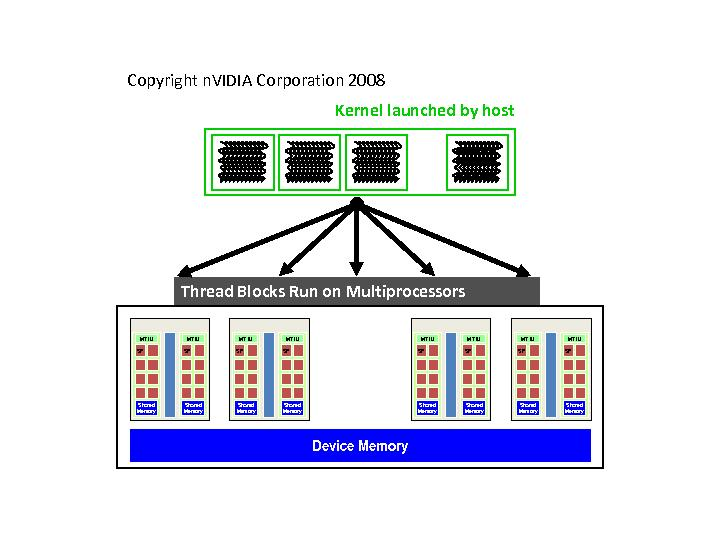
\includegraphics[width=\columnwidth]{figures/CUDADiagram}
\caption{NVIDIA GPU Diagram.  The CPU control thread launches a kernel with
  many threads per thread block.  Each thread block is assigned to a
  Multiprocessor (PE) containing 8 scalar processing elements and a local
  shared memory.  The Device Memory is global to all thread blocks; in
  pre-Fermi GPUs it was uncached.\vspace{-.20in}}
\label{fig:CUDAOrg}
\end{figure}

When calling a kernel, the user must specify the organization of threads into
thread blocks.  Tesla GPUs support up to 512 threads per block; Fermi
supports 1024.  A thread block will be allocated by the CUDA runtime system
to a particular PE on which it will execute.  To minimize SIMD overhead,
these threads are collected into smaller groups called {\em warps}.  Each PE
has a modest amount of very fast programmer controlled scratchpad memory,
denoted {\em shared memory}, which can be shared by threads in a thread block
but cannot be accessed by any other thread blocks.  For the purposes of this
paper, the only other memory structure available to threads running on the
GPU is a large global memory accessible by all threads on the device.

The CUDA model does not support any global synchronization primitive between
thread blocks during a kernel execution.  Instead, global synchronization
events require the completion of all running thread blocks and a return of
control to the CPU control thread.  A further complication is that no data
stored in the shared memory of a PE is persistent across kernel calls.
Global synchronization events are therefore very costly.

The implication of this model for stencil applications is that the kernel
author must be intimately familiar with the details of the CUDA runtime
system in order to organize work units into thread blocks in such a way that
usage of shared memory is maximized, and accesses to global memory are
minimized.  Key decisions in this allocation are the choice of tile size and
PH of the stencil calculation that the optimization model is designed to
make.  In order to accurately make such decisions, the allocator must be able
to predict the latencies of the various operations involved in the kernel's
calculations and memory accesses.

\subsection{SL CUDA Template}

In this section, we describe how our CUDA template code works.  This template
code is hand-written and hand-optimized by the SL implementers and does not
contain any application specific code.  The application specific code from
the SL specification is automatically merged into the template during the SL
translation process to generate the final ISL code.  The CUDA execution model
involves both a control thread on the CPU and kernel code that executes on
the GPU.  The CUDA template code includes both the CPU and GPU code needed to
support the application specific code provided by the SL user.

The primary function in the template is a C function for the CPU control
thread.  First, it calculates the tile size and the PH.  Then, it copies the
input matrix from system memory to GPU memory.  If an array of read-only data
is used, it also copies that data into GPU memory.  Finally, it runs a loop
in which it invokes the CUDA kernel to calculate the output matrix from the
input matrix.  It runs this loop for the specified number of iterations,
divided by the PH, or until convergence as determined by the execution of the
{\bf ConvergeValue} code block.

Each tile is processed by one CUDA thread block, and each cell in the tile is
owned by a single thread.  The input tile size will include GZ cells.  The
output tile size will be smaller.  The actual tile size used is determined at
application runtime using dynamically gathered information about the
execution environment.  For concreteness, consider a pre-Fermi CUDA card that
supports up to 512 threads per thread block.  In this case, the 3D input tile
will be $8 \times 8 \times 8$, the 2D tile $22 \times 22$, and the 1D tile
512 cells long.

The generated CUDA kernel includes both template code and application
specific code.  It operates as follows.  The thread calculates the $(x, y,
z)$ coordinates of the cell in the matrix that it owns.  It copies that
cell's value from the input matrix into the thread block's shared memory.
After each value has been copied into shared memory, the threads that own
cells in the outermost GZ sleep.  Those threads have completed their work.
Each other thread calculates the new value for its cell.  For each cell in
its stencil, the thread gets the cell value from shared memory.

If the PH is greater than one, then the threads continue running.  Each
thread copies the value that it just computed into shared memory.  Then, the
threads in the second outermost GZ sleep.  Their local copies of the
neighboring cell values in the outermost GZ are now out-of-date as their
values were calculated in an adjacent tile (see Figure~\ref{fig:trapezoid}).
The remaining threads calculate new values.  This process continues for the
number of iterations specified by PH.

When this process is complete, if a thread owned a cell that was not in the
GZ, then that cell copies the final value into device memory.  If a thread
owned a cell that was in the GZ, then that thread does not need to do
anything, since we are guaranteed that some thread in some other thread block
owned that same cell as part of its output tile, and that other thread will
own the responsibility to write the value into device memory.

Inside of the CUDA kernel, the program calls the user-specified {\bf
  CellValue} code to calculate new cell values, and it calls the
user-specified {\bf EdgeValue} code to get stencil values for cells along the
edges of the matrix.  All of the remainder of the kernel code is included in
the template in the SL template library.

\subsection{Pyramid Height Calculation}

As mentioned above, the performance of stencil applications on parallel
hardware is critically dependent on the proper relationship between tile size
and GZ size or PH.  To calculate the optimal PH, we extended and automated
the CUDA analytical model by Meng and Skadron.  They developed a complex
analytical model in MatLab that uses information from several sources to
calculate the expected program runtime.  Their model requires several pieces
of information as input.

First, it needs information about the stencil application itself.  Some
information is static, such as the data dimensionality, the stencil size
(GZ), the number of global memory accesses required during movement of tile
data into shared memory, and the number of global accesses for read-only data
required during each cell calculation.  Other information is dynamic, such as
the data set size and the number of instructions that each thread must
execute in the shared memory setup portion of the kernel and in the kernel
cell calculation.  Since they proposed but did not implement any code
annotations for the stencil applications, many of the application specific
parameters were hand coded in MatLab for the four particular test case
applications.  In addition, the instruction count was gathered using the CUDA
profiler on hand-coded implementations of the test applications, and fed to
the model by hand.

Second, the specific properties of the target GPU are important.  This
includes the number of PEs, the number of concurrent blocks that can run on a
PE, the number of threads allowed per block, the time required for the GPU to
perform a global synchronization, and several GPU memory performance
parameters.  These values were acquired by a number of means, including hand
coding some parameters based on the published characteristics of a few
specific models of GPU and by data regression of the runtimes from specific
applications.

The multi-node implementation using MPI and CUDA uses the stencil size to
determine the necessary border for each node.  While this correlates with the
concepts of the GZ and PH at the macro level, it is actually statically
calculable and does not impact the PH computation.  MPI sends the needed data
for the assigned elements to the relevant nodes.  Nodes return only the
calculated results to the root, which collates them to form the result matrix.

\subsubsection{Modification of Meng and Skadron Model}

We have modified and improved this model in several important ways.

First, we ported the model from MatLab to C++ to include it in the
application and allow it to perform the optimization at runtime.  This allows
gathering runtime information about the program in the current execution
environment, allowing it to be run on different GPUs without recompilation.
The resulting code is better optimized for the specific characteristics of
the particular hardware, not just the architectural features of the hardware.
While this means that the time to perform the optimizations is included in
the total runtime for the program, the difference in runtimes for the wrong
optimizations will generally dwarf the cost of calculating the optimizations
themselves.  In addition, stencil applications typically take many iterations
to converge, allowing more time over which to amortize the optimization
costs.

Second, the static and architecture-independent application specific
information about the dimensions of the data space, the stencil size, etc.,
now come directly from the SL program specification.  These are compiled into
the generated code for the ISL calculation.

Third, the remaining application-specific information is acquired dynamically
at runtime.  This includes the data set size, and the parameters that
previously came from profiling, such as the kernel thread setup time and cell
value calculation time.  The latter two numbers are acquired by running the
application with PH of 1 and 2. From these numbers, the setup and cell
calculation times are easily computed.  Currently we throw away the
application computation performed during these data gathering runs, but in
the future, the time spent gathering this information could result in the
completion of the first three iterations of the computation.

Fourth, the GPU device information is gathered through calls to various
functions provided in the CUDA runtime libraries.  In particular, we can
acquire the number of PEs, the concurrent blocks per PE, and the maximum
number of threads per block.  We can also query the CUDA runtime system for
the number of threads per block for the actual kernel of the running
application.  This can sometimes result in tighter restrictions on the
allowed threads per block if, for example, the kernel requires more resources
from the device than the architecture can provide.  This is particularly true
for CUDA kernels that use many of registers.  Knowing this information is
critical to optimization because, on the CUDA architecture, stencil
applications generally run faster with a larger tile size as long as the data
set size is large enough to saturate the number of available PEs.  Since the
threads-per-block count determines the tile size, knowing this number
precisely allows the optimizer to pick the largest tile size that the current
GPU can handle.  Future GPUs will likely allow the number of threads per
block to increase further; gathering this information at run time allows
generated code to calculate the optimal tile size for such cards without
recompilation.

Fifth, the time required for a global synchronization is acquired by running
a null kernel on the device with the same data set size parameters as are
required to run the actual kernel.

Finally, Meng and Skadron originally did a manual gradient descent on
runtimes to determine the best PH and tile size.  Since we can determine the
best tile size as described earlier, we do an automatic gradient descent
starting at PH of 1, and continue calculating the model latency until it is
higher than the previous one, then use that PH for the remainder of the
application iterations.

\section{Experimental Results}\label{sec:results}

Our primary emphases are the definition of a stencil language, providing a
source-to-source compiler for it, and optimizing the generated programs in
terms of GPU shared memory, tile size, and PH with an extension of the
analytical model of Meng and Skadron.  The availability of the Fermi and
Tesla architectures presents an opportunity to test the robustness to
architectural changes of our model enhancement which utilizes
dynamically-collected information about the execution environment.
Therefore, we present results for a GTX 480 (Fermi) and a GTX 280 (Tesla).

All runtimes include the CPU and GPU latencies for the ISL loop only.  The
time required to create and initialize arrays, and transfer arrays between
main memory and the GPU global memory are not included to allow us to focus
on the factors affecting the ISL performance.  In addition, the reported
runtimes for the SL optimized ISLs do not include the overhead needed to run
the optimizer.  Instead, the times are for the entire ISL loop running with
the parameters determined by the optimizer.  As stated above, the costs for
running the optimizer are fixed, so the overhead for the optimizer as a
percentage of the overall runtime can be arbitrarily large or small depending
on the number of iterations in the actual ISL loop.

We use the arithmetic mean when aggregating results and a SERPOP analysis
strategy (see~\cite{Mashey} for details).

Our GTX 480 is in a machine with an Intel Core2 Quad Q9400 clocked at 2.66
GHz with 3 MB L2 and 4 GB DRAM running Linux 2.6.32.  The 280 is attached to
dual Intel Core2 Extreme X9770 processors running at 3.2GHz with 6MB of L2
cache and 4GB of DRAM running Linux 2.6.24.  Both machines are running CUDA
3.1.  The 480 can manage 1024 threads per block with 60 PEs each with 8 SIMD
cores running at 1.4 GHz.  It has 2 GB of memory.  The 280 has 30 PEs, each
with 8 SIMD cores that handle up to 8 concurrent running blocks with a 512
thread maximum block size.  It is clocked at 1.3 GHz with 1 GB of global
memory.  All code was compiled with the NVIDIA NVCC compiler which calls GNU
tools (version 4.2.4) for compiling C++ code and linking.  All code was
compiled with -O3.  Our generated optimized code is based on hand optimized
templates, and thus is essentially equivalent to hand optimized code.

For our first test cases, we use the same four stencil applications as Meng
and Skadron did in their original study.  They are described below.  All of
the graphs of runtimes versus PH have the same basic curve.  Very low PHs are
not large enough to take advantage of all available spatial and temporal
locality, and perform worse than larger PHs, especially given the relatively
large cost of global synchronizations in the CUDA architecture.  However,
beyond some optimal PH, the runtimes again increase due to the overhead of
the redundant local GZ value calculations.  Another way to view this
trade-off is that with increased PH, the number of threads per tile that
calculate final cell values drops off at twice the size of the stencil per
dimension per step in PH (see Figure~\ref{fig:trapezoid}); therefore, for
larger PHs the effective tile size gets smaller, and the total number of
tiles---and therefore also the total number of threads---increases.
Eventually, in the limiting case, the PH is so high that {\em no} useful cell
values are calculated.  For these reasons, all of the graphs of runtimes
versus PH will be bowl shaped.  To better highlight the important portions of
the curves near the optimal---the minimum of the respective curve---PH, in
the following graphs we have not shown the extreme values at very high PH.
Furthermore, we present results for both the Fermi and Tesla architectures;
however, as the results are generally quite similar, we only include graphs
for Fermi.  Differences in results are discussed in the text.

\subsection{\em ``Pathfinder''}

The first test case is a 1D stencil application called {\em ``Pathfinder''}
that performs a dynamic programming calculation of the lowest cost of any
vertical path through a 2D grid.  The 2D input data set is read-only data in
the {\bf CellValue} computation.  Each loop iteration calculates the minimum
costs down another row in the 2D grid.  The tiles are horizontal slices
across the columns of the grid.  A valid path is one which varies by at most
one cell in each step from row to row, thus the stencil size is 1.
Figure~\ref{fig:pathfinderTimes} shows the Fermi runtimes versus PH for
Pathfinder for row widths of 100 k, 400 k, 700 k, and 1000 k.  As with all
the applications, these large sizes are chosen to ensure that the GPU is
computationally saturated.  The PH can range from 1 to 255 on Tesla and 1 to
511 on Fermi.

Notice that the valley for the main portion of this curve is very shallow.
Therefore, it is hard for the model to accurately predict the exact best PH.
And in fact, our model does not.  The measured best PH is 16 for all data set
sizes.  However, our optimizer predicts 61, 24, 24, and 25 for the 100 k, 400
k, 700 k, and 1000 k data set sizes and resulting in performance loses of
only 12\%, 2.6\%, 0.7\%, 1.2\%, respectively.  Tesla results are similar,
with a performance loss of 5.8\% for the 400 k dataset and less than 1\% for
all others.  From these results, one can see that the shape of the
interesting part of the curve is so flat that precise PH prediction is not
necessary to achieve very positive results.  For comparison, the poor choice
of a PH of 1 for the 400 k column data set would result in a performance loss
of nearly $2.5\times$.
\begin{figure}
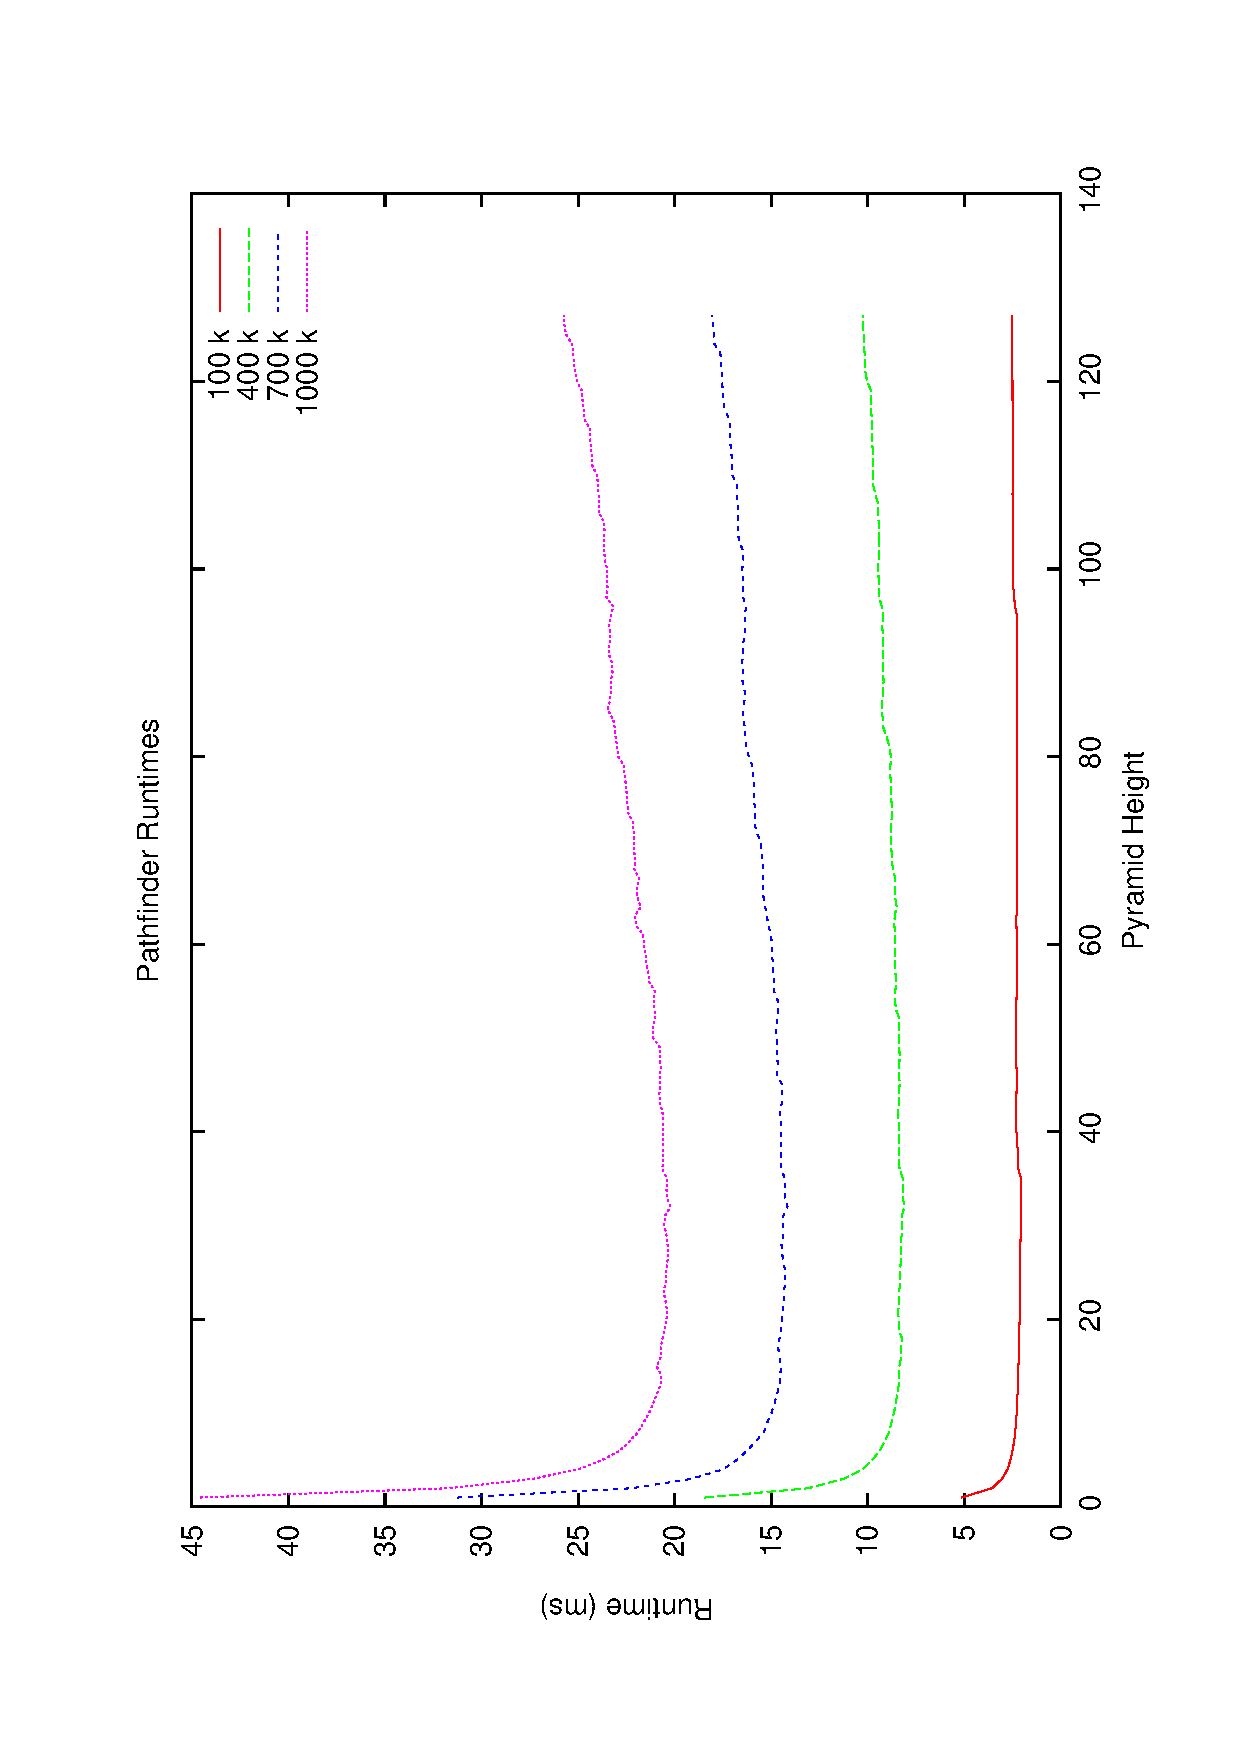
\includegraphics[angle=270,width=\columnwidth]{figures/path}
\caption{Fermi runtimes for the Pathfinder 1D application versus PH.  The lowest
  portion of the curves are very flat.  Therefore, even though our model did
  not pick the optimal PH for any data set size, performance was still near
  optimal.\vspace{-.20in}}
\label{fig:pathfinderTimes}
\end{figure}

\subsection{\em ``HotSpot''}
The second test case is a 2D stencil application called {\em ``HotSpot''}.
The stencil language description for this application is shown in
Figure~\ref{fig:hotspot}.  The application solves a series of ordinary
differential equations that model heat dissipation in a conductive material,
the silicon substrate of a computer chip~\cite{hotspot}.  On each time step
of the computation, the heat generated by the chip components propagates
through the modeled substrate.  This is constant read-only data read for each
cell on each iteration.  As this is a 2D application, the theoretical maximum
square tile size on a Fermi board is 32x32, and 22x22 on Tesla implying
possible PH ranging from 1--15 and 1--10, respectively.  The Fermi runtimes
versus PH are show in Figure~\ref{fig:hotspotTimes}.  As can clearly be seen,
for the four data set sizes, the optimal PH is 2; this also holds true for
Tesla.  That is also the height calculated by our optimizer.
\begin{figure}
\includegraphics[angle=270,width=\columnwidth]{figures/hs}
\caption{Fermi runtimes for the HotSpot 2D stencil application versus PH.  As can
  be seen, the curve is bowl shape with a minimum at PH 2.  The effect is
  more pronounced with greater data set sizes.  Our optimizer picked the
  correct PH of 2 for all these data sets.\vspace{-.20in}}
\label{fig:hotspotTimes}
\end{figure}

\subsection{\em ``Plate''}
The third test case is a 2D stencil application called {\em ``Plate''}.  It
is very similar to and replaces the {\em ``Poisson''} application from the
original test suite.  It also models heat transfer in a plate but this time,
the heat injection into the system is modeled as coming from the edge of the
plate, not distributed throughout.  This differentiates the application from
HotSpot in two important ways.  First, there is no required read of global
data in each time step.  Second, it gives us an opportunity to use the {\bf
  EdgeValue} capability of SL to inject the heat at the plate's edge.  Again
the maximum square tile sizes are 32x32 and 22x22 and valid PHs are 1--15 and
1--10 for Fermi and Tesla, respectively.  The Fermi model predicted optimal
PHs of 4, 3, 3, and 3 for the $500^2$, $1000^2$, $1500^2$, $2000^2$ stencils,
respectively, and the Tesla model predicted optimal PH or 2 across the board.
All predictions were accurate.  As the results for Plate are so similar to
HotSpot, we don't include a graph.

\subsection{\em ``Cell''}
The fourth test case is a 3D stencil application called {\em ``Cell''}.  It
models Conway's Game of Life in 3 dimensions.  In each time step, each cell
calculates whether it is alive or dead based on the number of neighboring
cells that were alive in the previous time step.  To perform this
calculation, it looks at its 26 nearest neighbors.  For a 3D application, the
maximum tile size on Tesla is 8x8x8, and 10x10x10 on Fermi, and the possible
PHs are only 1--3 and 1--4, respectively.  The Fermi runtimes versus PH are
shown in Figure~\ref{fig:cellTimes}.  It is clear from the chart that a PH of
3 or 4 is a very bad choice.  The runtimes for PHs of 1 and 2 are similar,
but 1 is better and is also correctly predicted by our model in all cases for
Tesla and in all but the $40^3$ case on Fermi, which predicted an optimal PH
of 2.
\begin{figure}
\includegraphics[angle=270,width=\columnwidth]{figures/cell}
\caption{Fermi runtimes for the Cell 3D stencil application versus PH.  The
  curve shows that a PH of 3 or 4 is a very bad choice.  While the values for
  1 and 2 are slightly compressed in the graph, the optimal PH is in fact 1
  for all data sets.\vspace{-.20in}}
\label{fig:cellTimes}
\end{figure}

\subsection{Model Comparisons}
As we have demonstrated, our model predicts the optimal PH for HotSpot,
Plate, and Cell (save one instance out of eight) on Fermi and Tesla.  These
were the same PHs predicted by the original model of Meng and Skadron for
these same applications and data set sizes; however, they measured an optimal
PH of 3 for HotSpot and Poisson.  Their implementation differs from ours in
two important ways.

First, their implementations took advantage of architectural details that are
not exposed to users of SL, allowing them to load the read-only heat data
used in HotSpot into shared memory to take advantage of temporal locality.
Our SL has no way for the application programmer to express the access
patterns for read-only data, and therefore our version of HotSpot will read
the value from global memory in each time step.  The ability of
hardware-tuned code to reuse the global memory read across several time steps
tends to drive the optimal PH higher, leading to greater temporal reuse of
data values loaded into shared memory.  We hope to add better support for
read-only data to SL at a future date.

Second, their inner loop code calculates the cell values for all cells in the
tile, even those that have become too far away from the center of the tile to
matter to the computation.  Another option is to recalculate the zone of
cells involved in useful computation on each time step.  This keeps threads
from calculating values that will never be used at the cost of more GZ size
calculations.  Given that our system must access read-only data from global
memory in HotSpot---and potentially in other applications---the strategy of
recalculating the GZ size in each time interval mitigates the number of
global reads required, and is therefore the correct choice for such
applications.

We found that 2D and 3D applications run faster by restricting the number of
calculated values, even without using read only data. We believe this is
because whole thread warps on the top and bottom of the tile will only have
to check on each time step if they are still calculating useful values.  In
3D applications, this effect is even more pronounced as warps in the front
and back of the tile have this same advantage.  The GZs on the sides of the
tile tend not to span entire warps, so there is no advantage for warps at the
sides of the tile from this effect, while the GZs in a 1D application only
grow on the sides.  Our CUDA templates take advantage of these effects by
continuing to calculate values in the GZ for 1D stencil applications, but not
for 2D or 3D applications.  As a result of this change, our Pathfinder
runtimes were significantly reduced.

\begin{figure}
\includegraphics[angle=270,width=\columnwidth]{figures/hs_pred}
\caption{Fermi runtimes for HotSpot versus normalized runtimes predicted by
  the Model for PHs from 1 to 6.  While the shape of the model curve does not
  precisely match that of the measured runtimes, the model accurately
  predicts an optimal PH of two.\vspace{-.20in}}
\label{fig:modelvsactual}
\end{figure}

We also analyzed the actual runtimes versus our model predictions.
Figure~\ref{fig:modelvsactual} shows HotSpot runtimes on Fermi versus
predictions for PHs from 1 to 6.  The model predictions are in terms of GPU
cycles, not runtimes.  Therefore, the model times are normalized to the
actual runtime at the optimal PH of 2.  This allows a more direct comparison
of the relative curves shapes, which is more important than absolute scaling
for choosing the optimal PH.  As the figure shows, the model has a steeper
bowl shape than the actual runtimes.  The effect is more pronounced for
higher PHs, and grows large quickly for PHs between 6 and 10 which are
truncated to better show the most interesting part of the curves.

The results presented here validate that the changes that we have made to the
CUDA ISL analytical model have not lessened the effective accuracy of its PH
predictions.  Given the advantage of the elimination of the users' manual
involvement in this optimization, we believe this to be an important
contribution of this work.

\subsection{Comparison to Na\"{i}ve CUDA code}

\begin{figure}
\resizebox{\columnwidth}{!}{
\begin{tabular}{|l||c|c|c|c|c|c|}
\hline

{\bf Application} & {\bf Pathfinder} & {\bf Plate} & {\bf PlateHalo} & {\bf
  Plate++} & {\bf HotSpot} & {\bf Cell} \\
\hline

\multicolumn{7}{|c|}{Fermi}\\
\hline
\hline

Data Set Size	& 400K	& $1000^2$	& $1000^2$	& $1000^2$	& $1000^2$	& $60^3$	\\
\hline

Source of Best Time & O PH=32 	& SL PH=3	& SL PH=3	& SL PH=2	& SL PH=2	& SL PH=1	\\

Oracle		& 8.3 ms	& 61.4 ms	& 66.7 ms	& 85.9 ms	& 78.0	ms	& 16.0 ms	\\

SL Optimized vs Na\"{i}ve & 2.06 & 1.17		& 1.54		& 1.26		& 1.11		& 1.44		\\

SL Optimized Time & 8.6 ms	& 61.4	ms	& 66.7	ms	& 85.9	ms	& 78.0	ms	& 16.0	ms	\\

SL PH=1		& 18.4	ms	& 81.3	ms	& 85.1	ms	& 91.9	ms	& 95.8	ms	& 16.0	ms	\\

Na\"{i}ve	& 17.7	ms	& 71.8	ms	& 102.8 ms	& 108.0 ms	& 86.3	ms	& 23.0	ms	\\

\hline

\multicolumn{7}{|c|}{Tesla}\\
\hline
\hline

Source of Best Time & O PH=16 	& SL PH=2	& SL PH=2	& SL PH=1	& Na\"{i}ve	& SL PH=1	\\

Oracle		& 9.4 ms	& 114.2 ms	& 131.8 ms	& 176.3 ms	& 141.0 ms	& 36.5 ms	\\

SL Optimized vs Na\"{i}ve & 2.37 & 1.09		& 1.82		& 1.26		& 0.97		& 2.37		\\

SL Optimized Time & 9.7 ms	& 114.2 ms	& 131.8 ms	& 176.3 ms
& 145.3 ms	& 36.5  ms	\\

SL PH=1		& 23.6	ms	& 145.1 ms	& 160.1 ms	& 176.3 ms	& 162.9 ms	& 36.5	ms	\\

Na\"{i}ve	& 23.0	ms	& 124.9 ms	& 239.7 ms	& 222.0 ms	& 141.0 ms	& 86.6	ms	\\

\hline

\end{tabular}
}

\caption{Runtimes for the SL optimized code for the four applications in
  Section~\ref{sec:results}, plus two new versions of Plate.  Runtimes are
  also shown for a na\"{i}ve CUDA implementation, along with a comparison
  relative to SL optimized code.  For applications with large amounts of
  either temporal or spatial locality, the SL generated code far outperforms
  the na\"{i}ve code.  For other applications, the difference is more modest.
  Data are listed for Fermi, on the top of the table, and Tesla, on the
  bottom.  Fermi's larger block size results in higher optimal PH for Plate,
  PlateHalo, and Plate++ due to the larger tile sizes.  The inclusion of a
  cache on Fermi also results in a lower relative improvement of SL optimized
  code versus na\"{i}ve for applications with large amounts of temporal or
  spatial locality.\vspace{-.20in}}
\label{fig:table}
\end{figure}

In judging the performance of optimized code, it is important to see the
effects of the optimizations compared against code that does not have those
optimizations.  Table~\ref{fig:table} shows where we compare a ``na\"{i}ve''
CUDA implementation of the four applications discussed above along with two
additional applications.

The na\"{i}ve CUDA implementation does not use shared memory.  Instead,
global device memory is always accessed.  Therefore, each PE can only
calculate one time step before synchronizing with neighboring PEs.  While
there are some edge cases to consider at the boundaries of the data set,
there is no longer any need to handle edge cases across internal tile
boundaries.  The na\"{i}ve code does still benefit from large tile sizes; the
maximum possible sizes are used.  Overall, this code is much simpler than the
optimized code, and approximates what an inexperienced CUDA programmer would
produce.

The also shows the runtimes of the SL generated code, but with PH=1.
Finally, the table also shows the runtime of the SL generated code with an
oracle selecting the best code.  This often matches the SL optimized code,
but differs in those cases where SL does not accurately predict the best PH,
and the one case where the na\"{i}ve code outperforms the SL generated code.

We can see from the table that the SL generated code outperforms the
na\"{i}ve code by between $2.37\times$ and $0.97\times$ with an arithmetic
mean of $1.65\times$.  The SL optimized code outperforms the na\"{i}ve code
by a significant factor for both the 1D Pathfinder application, and the 3D
Cell application, but for different reasons.  In Pathfinder, the optimal PH
are high at 32 and 16, so there is substantial temporal reuse of the data
values stored in shared memory even though the spatial reuse is limited by
the single dimension of the data.  This is further seen by looking at the
PH=1 runtime for the SL code.  By setting the PH=1, all of the temporal reuse
is eliminated, and the overhead of the additional complexity of the SL code
causes it to run slightly slower than the na\"{i}ve code.

On the other hand, in Cell, the stencil involves 26 neighboring cell values.
So, even though the temporal reuse is non-existent with an optimal PH of 1,
the spatial reuse is significant.  In the 2D applications, the optimal PH of
Plate and HotSpot are always small, and the stencil involves only 4 adjacent
cells, so neither the spatial nor temporal reuse is extremely high.  In fact
the na\"{i}ve code runs faster than SL's optimal code for HotSpot on Tesla,
as the latter is also doing global memory reads in each time step.

To further explore these issues, we added two additional versions of Plate to
our study.  The first,{\em PlateHalo}, expands the number of adjacent cells
used in the computation to 8 by including the diagonal neighbors.  This
increases the spatial locality of the data in shared memory, and we see that
the runtime for the na\"{i}ve version increases significantly in PlateHalo
over Plate, while the SL optimized version shows only a modest change in
performance.

The second variation of Plate is called {\em Plate++}.  It also expands the
stencil to include 8 neighbors, but this time by going out 2 cells to the
north, south, east, and west.  As this causes the GZs to grow twice as fast
as in Plate, the optimal PH are now 1 and 2.  Temporal reuse is
reduced---eliminated on Tesla---in the SL code, and SL code for Plate++ runs
slower than either Plate or PlateHalo.  The na\"{i}ve code for Plate++ runs
8\% faster than the na\"{i}ve code for PlateHalo on Tesla, perhaps because of
better memory access coalescence, or fewer memory bank conflicts.

\subsection{Multinode CUDA with MPI}

\begin{figure}
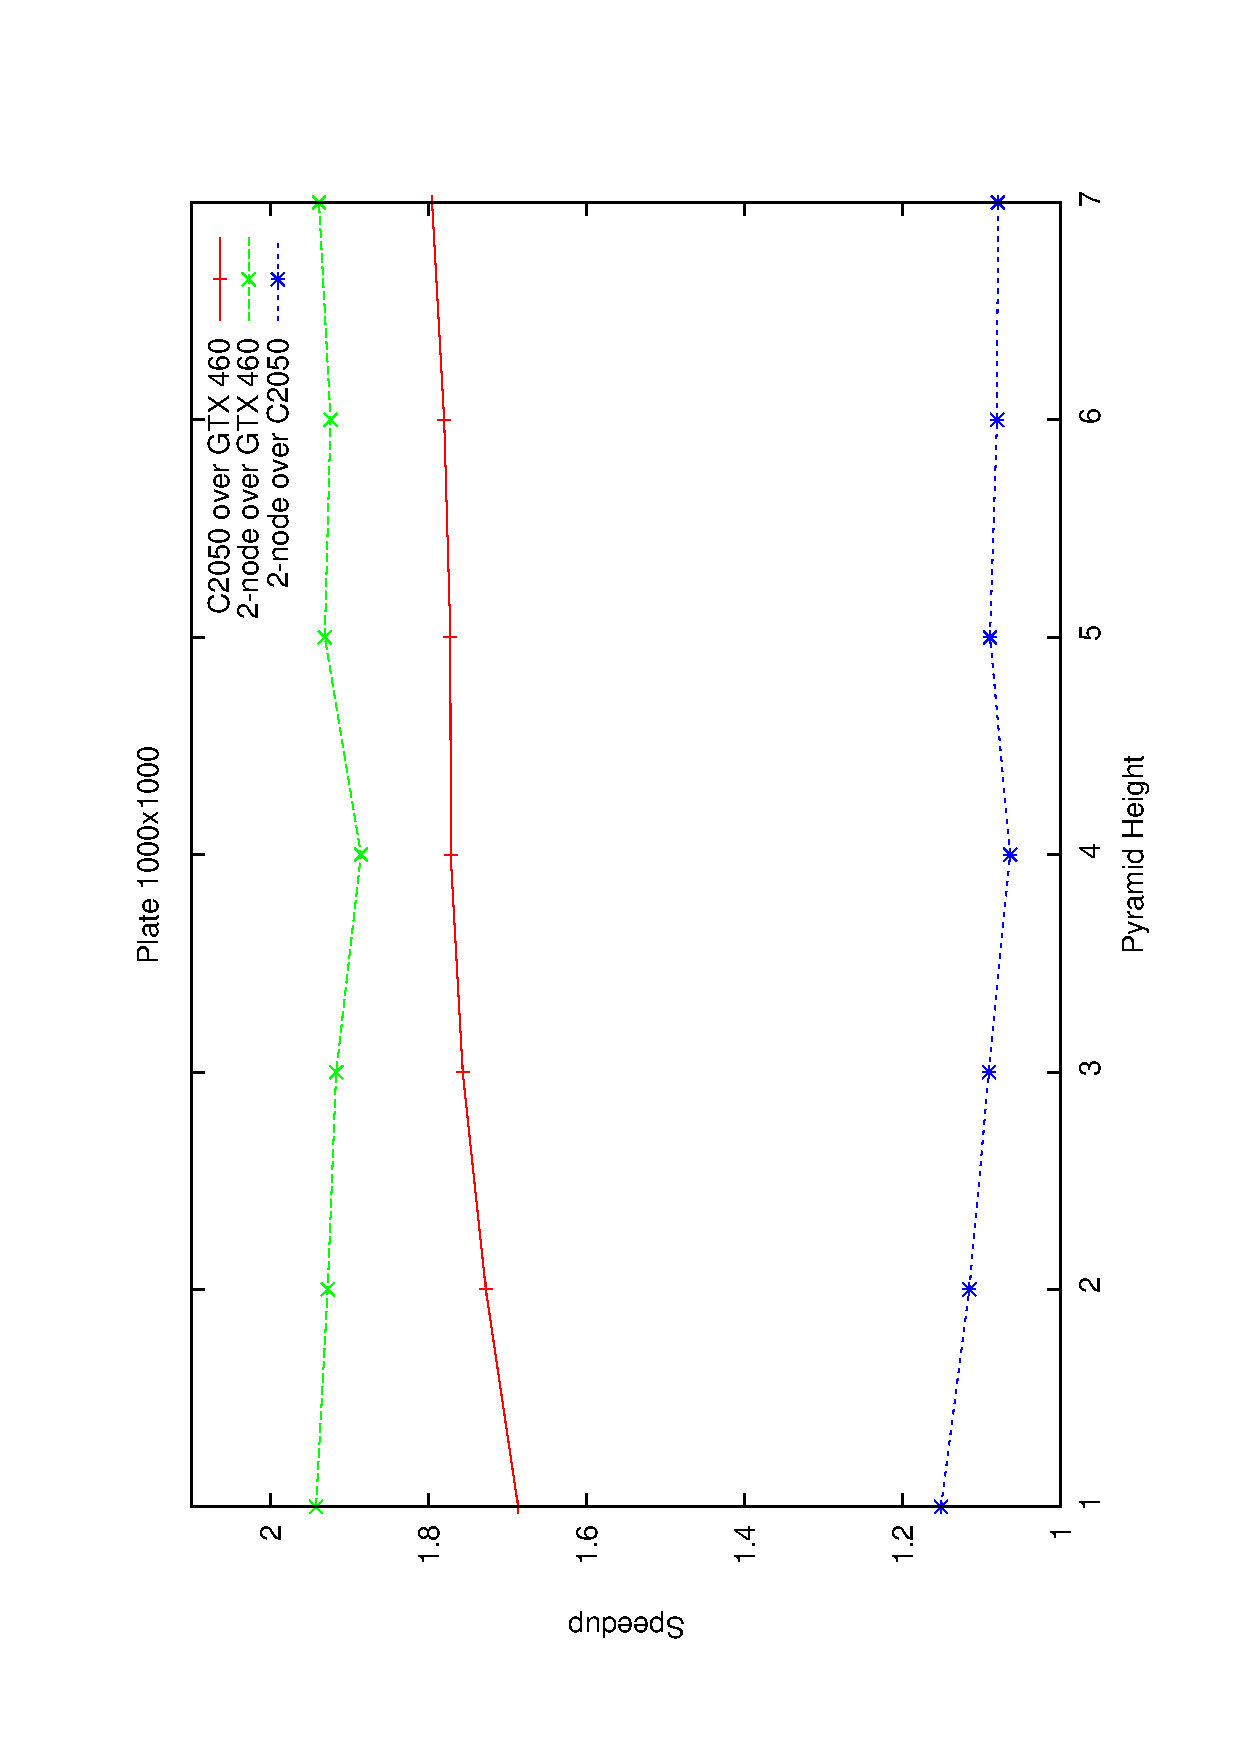
\includegraphics[angle=270,width=\columnwidth]{figures/2-node}
\caption{2-node performance for Plate at $1000\times 1000$ using a GTX 460
  and a C2050.  The speedup for the C2050 over the GTX 460 is also included
  to give a sense of the performance differences of the parts.
\label{fig:2-node}\vspace{-.20in}}
\end{figure}

Our MPI implementation does not account for non-heterogeneous
distribution of GPUs, nor do we have machines with matching hardware such
that we can do a complete, fair performance evaluation of a multinode GPU
cluster.  We present multinode results to show proof of concept and that even
a na\"ive multinode implementation on a non-heterogeneous cluster will
provide performance benefits.

Figure~\ref{fig:2-node} shows the speedup of a heterogeneous 2-node cluster
over it's constituent nodes, one running a GTX 460 and the other a Tesla
C2050.  The figure also shows the speedup of the 2050 over the 460 to give an
idea of the relevant performance differences of the parts.  Other benchmarks
demonstrate similar results.  This figure shows that optimal pyramid height
is independent of multinode computation, at least until working sets become
so small that communication dominates.

\section{Related Work}

Li et al.\ may have been the first to use the term {\em iterative stencil
  loops}~\cite{li}.  They developed a compiler framework for these loops that
used tiling to improve temporal data locality.  Their work was intended to be
run on a uniprocessor, so they did not face any communication costs and they
did not consider ghost zones.

We are not the first to create a stencil compiler.  Brickner et al.\ created
a stencil compiler for the Connection Machine CM-2 massively parallel
architecture~\cite{cm2}.  The stencil expression was expressed in microcode
which was specific to the CM-2.  Other recent stencil compilers are
Pochoir~\cite{DBLP:conf/spaa/TangCKLL11} and PATUS~\cite{10.1109/IPDPS.2011.70}.  Our framework is distinguished
from these by the inclusion of MPI and by our runtime optimizations.

In parallel with our efforts, Orchard et al.~\cite{ypnos} have developed a
stencil language called {\em Ypnos} as an extension to Haskell.  They also
argue for an architecture-independent declarative language for ISLs, and as
in SL, rely on language features instead of complex program analysis to
determine the size and shape of the stencils and data.  Their language
includes reduction operators as a means of specifying convergence criteria,
and they allow users to explicitly specify a PH for an ISL computation but do
not support automatic PH optimization.  They do not report Ypnos performance
results.

Kamil et al.~\cite{kamil} studied the effects of tile size and time skewing
on memory locality on Itanium2, Opteron, Power5, and Cell.  They concluded
that controlling tile size, temporal locality across time slices, and
hand-tuned control of scratchpad memory is critical to performance.  We
optimize use of CUDA's scratchpad memory, tile size, and temporal reuse;
however, our temporal locality is always strictly in the time dimension, as
we have not investigated the use of time skewing.  Datta et
al.~\cite{AutoTuning} studied optimizations for stencil applications across a
wide range of architectures including CUDA.  Their optimizer uses auto-tuning
to find optimal solutions, as does another paper by Kamil et al~\cite{5470421}.  Our analytical model starting point allows our
training period to be very short relative to a typical ISL computation.

Micikevicius explored hand coding stencil applications for CU\-DA, and ghost
zone sizes~\cite{Micikevicius}.  They also explored using asynchronous data
transfers for data sets too large to fit in GPU global memory.  Volkov et
al.\ explored hand optimizing CUDA programs involving parallel operations on
large arrays~\cite{volkov}.  We have included a subset of the optimizations
presented by Micikevicius and Volkov in our CUDA template library, but we
have no support for arrays too large to fit into the device's global memory,
and therefore we did not investigate asynchronous data transfers.

Several attempts have been made to build simplifying layers on top of CUDA.
Lee et al.\ implemented a source-to-source translator for OpenMP to
CUDA~\cite{openmp2gpu}.  OpenMP can express a significantly wider range of
parallel computations then can be expressed by SL; however, this also means
an OpenMP translator cannot include stencil application specific
optimizations as we do.  There is also previous work similar in nature to the
pyramid height optimization including work by Bassetti et
al.~\cite{Bassetti:1998:OTS:646894.709707} and Nguyen et
al~\cite{Nguyen:2010:BOS:1884643.1884658}.

CUDA-lite is a general purpose, source-to-source translator for automatically
optimizing CUDA programs~\cite{cudalite}.  The user specifies a na\"{i}ve
CUDA implementation of their ISL that only uses global memory, and adds some
pragmas that give hints about the size, shape, and data access patterns.
Then CUDA-lite generates an optimized CUDA program that leverages the
specialized memory spaces, resulting in 2--$17\times$ speedups for their test
applications.  It appears they ran their tests on earlier GPUs that had less
flexible memory access coalescing hardware than modern GPUs.  In addition,
their primary test applications were not stencil applications, and instead
performed operations such as matrix multiply. These contain large amounts of
spatial and temporal locality, and are compute intensive, allowing for more
processing time to hide memory access latency~\cite{Ryoo}. By comparison, SL
also optimizes for shared memory but not texture memory, and also optimizes
PH.

\section{Conclusions and Future Directions}

We have defined a new language, SL, for easily expressing stencil
applications.  SL is a formal, high-level language in which a programmer can
conveniently describe an ISL computation by focusing on the simple
computation needed to compute cell values.  No optimization nor
architecture-specific information is needed.

We have created an SL compiler that uses templates to allow the generated
code to be extended to many parallel execution environments.  Based on a
single source file, it generates efficient code for CUDA, OpenMP and MPI;
other environments are possible.  SL's architecture allows
targeting of languages which are not C-like; Fortran, for example, which is
still quite popular for high-performance computing.

We have implemented an initial template and an optimizer for the CUDA
programming environment that blocks computations to use the scratchpad
memory, and that estimates the best PH.  The optimizer is fully automatic and
utilizes both static and dynamic application information.  It accurately
calculates the optimal tile size and PHs for most applications, on both Tesla
and Fermi class GPUs.  As a result, with an SL source of about 16 lines, a
user can achieve average speedups of $1.65\times$ for the GTX 280, and
$1.43\times$ for the GTX 480, over na\"{i}ve CUDA code.  Yet the SL
specification is much easier to write than even the na\"{i}ve CUDA code, and
is similar to writing code for a single thread CPU.

The optimizer's ability to leverage dynamically acquired information about
the runtime environment means that the generated code can be used on a
variety of devices.  Our model ported directly from its original the Tesla
target to the Fermi architecture with only trivial modification.

The current SL architecture can be extended in several directions.  First,
with language extensions, we can improve support for read-only data at least
in the common cases, such as HotSpot, where the array access pattern is
straightforward.  A second SL language extension could add support for
reduction operators and ISL termination based on a data convergence criteria.
It would also be interesting to investigate data morphing as a way to improve
cache performance or reduce memory bank conflicts.

\section*{Acknowledgements}
This work was supported in part by NSF grant CNS-0916908 and by a grant from
NEC Research Labs America.

%\acks

%Acknowledgments, if needed.

% We recommend abbrvnat bibliography style.

%\addtolength{\itemsep}{-0.2\baselineskip}
\balance
\bibliographystyle{IEEEtran}
\bibliography{PPoPP-report}

\end{document}
